\begingroup
\begin{figure}[!htb]
    % \setArraystrech{1.5}
    \setlength\tabcolsep{0pt}
    \centering
    \begin{tabular*}{\textwidth}{ c c c c  c c c c  c }
        Target & Output & Normal & Voxel  &  Target & Output & Normal & Voxel & \\
        %%%%%%%%%%%%%%%%%%%%%%%%%%%%%
        %%%%% GUITARS & HOTDOGS %%%%%
        %%%%%%%%%%%%%%%%%%%%%%%%%%%%%

        %%%%% GUITARS_EXVA %%%%%
        &
        \begin{tabular}{cc}
            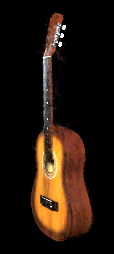
\includegraphics[width=0.062\textwidth]{figures/results/stat_set/valid/guitar4_exva_89k.png} & 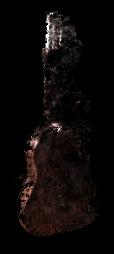
\includegraphics[width=0.062\textwidth]{figures/results/stat_set/valid/guitar8_exva_89k.png}
        \end{tabular}
        &
        \begin{tabular}{cc}
            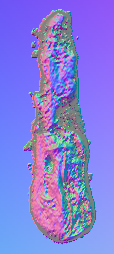
\includegraphics[width=0.062\textwidth]{figures/results/stat_set/valid/guitar4_exva_normal_89k.png} & 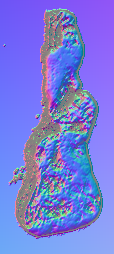
\includegraphics[width=0.062\textwidth]{figures/results/stat_set/valid/guitar8_exva_normal_89k.png}
        \end{tabular}
        &
        \begin{tabular}{cc}
            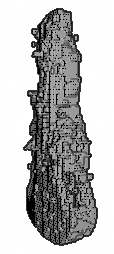
\includegraphics[width=0.062\textwidth]{figures/results/stat_set/valid/guitar4_exva_voxel_89k.png} & 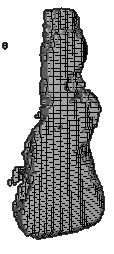
\includegraphics[width=0.062\textwidth]{figures/results/stat_set/valid/guitar8_exva_voxel_89k.png}
        \end{tabular}
        &
        %%%%% HOTDOG_EXVA %%%%%
        &
        \begin{tabular}{cc}
            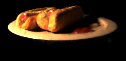
\includegraphics[width=0.124\textwidth]{figures/results/stat_set/valid/hotdog8_exva_55k.png} \\[-6pt]
            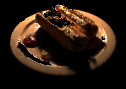
\includegraphics[width=0.124\textwidth]{figures/results/stat_set/valid/hotdog10_exva_55k.png}
        \end{tabular}
        &
        \begin{tabular}{cc}
            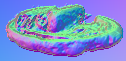
\includegraphics[width=0.124\textwidth]{figures/results/stat_set/valid/hotdog8_exva_normal_55k.png} \\[-6pt]
            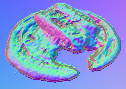
\includegraphics[width=0.124\textwidth]{figures/results/stat_set/valid/hotdog10_exva_normal_55k.png}
        \end{tabular}
        &
        \begin{tabular}{cc}
            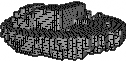
\includegraphics[width=0.124\textwidth]{figures/results/stat_set/valid/hotdog8_exva_voxel_55k.png} \\[-6pt]
            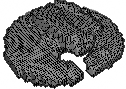
\includegraphics[width=0.124\textwidth]{figures/results/stat_set/valid/hotdog10_exva_voxel_55k.png}
        \end{tabular} 
        &
        \rot{ExVA}
        \\[-5pt]

        %%%%% GUITARS_NSVF %%%%%
        \begin{tabular}{cc}
            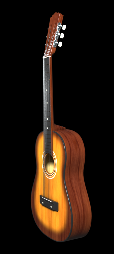
\includegraphics[width=0.062\textwidth]{figures/results/stat_set/valid/guitar4_targ_256px.png} & 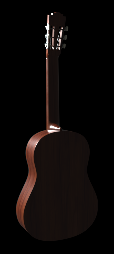
\includegraphics[width=0.062\textwidth]{figures/results/stat_set/valid/guitar8_targ_256px.png}
        \end{tabular}
        &
        \begin{tabular}{cc}
            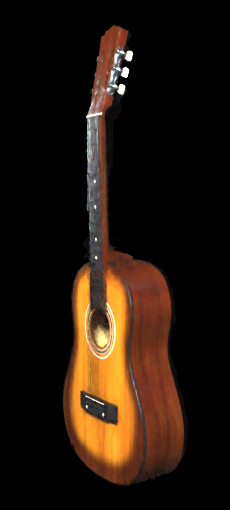
\includegraphics[width=0.062\textwidth]{figures/results/stat_set/valid/guitar4_nsvf_119k.png} & 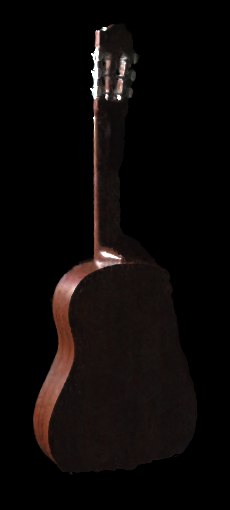
\includegraphics[width=0.062\textwidth]{figures/results/stat_set/valid/guitar8_nsvf_119k.png}
        \end{tabular}
        &
        \begin{tabular}{cc}
            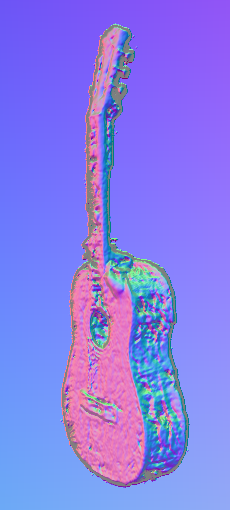
\includegraphics[width=0.062\textwidth]{figures/results/stat_set/valid/guitar4_nsvf_normal_119k.png} & 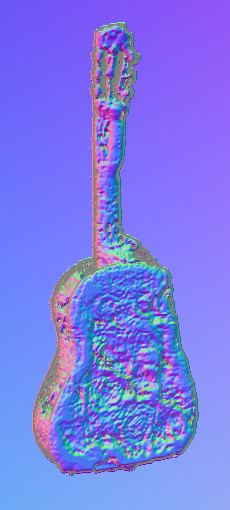
\includegraphics[width=0.062\textwidth]{figures/results/stat_set/valid/guitar8_nsvf_normal_119k.png}
        \end{tabular}
        &
        \begin{tabular}{cc}
            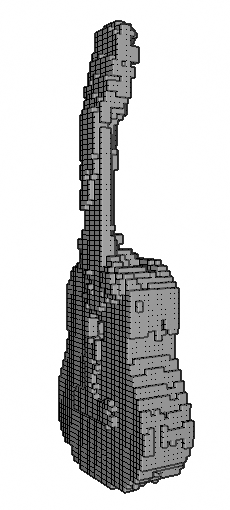
\includegraphics[width=0.062\textwidth]{figures/results/stat_set/valid/guitar4_nsvf_voxel_119k.png} & 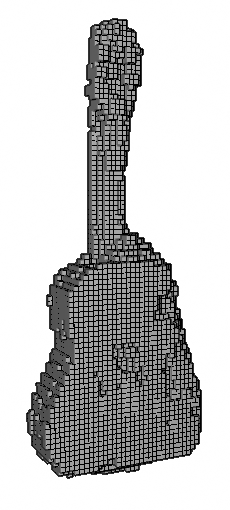
\includegraphics[width=0.062\textwidth]{figures/results/stat_set/valid/guitar8_nsvf_voxel_119k.png}
        \end{tabular}
        &
        %%%%% HOTDOG_NSVF %%%%%
        \begin{tabular}{cc}
            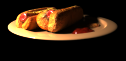
\includegraphics[width=0.124\textwidth]{figures/results/stat_set/valid/hotdog8_targ_128px.png} \\[-6pt]
            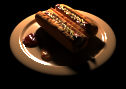
\includegraphics[width=0.124\textwidth]{figures/results/stat_set/valid/hotdog10_targ_128px.png}
        \end{tabular}
        &
        \begin{tabular}{cc}
            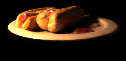
\includegraphics[width=0.124\textwidth]{figures/results/stat_set/valid/hotdog8_nsvf_57k.png} \\[-6pt]
            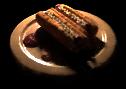
\includegraphics[width=0.124\textwidth]{figures/results/stat_set/valid/hotdog10_nsvf_57k.png}
        \end{tabular}
        &
        \begin{tabular}{cc}
            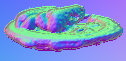
\includegraphics[width=0.124\textwidth]{figures/results/stat_set/valid/hotdog8_nsvf_normal_57k.png} \\[-6pt]
            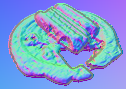
\includegraphics[width=0.124\textwidth]{figures/results/stat_set/valid/hotdog10_nsvf_normal_57k.png}
        \end{tabular}
        &
        \begin{tabular}{cc}
            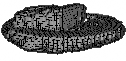
\includegraphics[width=0.124\textwidth]{figures/results/stat_set/valid/hotdog8_nsvf_voxel_57k.png} \\[-6pt]
            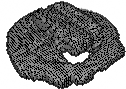
\includegraphics[width=0.124\textwidth]{figures/results/stat_set/valid/hotdog10_nsvf_voxel_57k.png}
        \end{tabular} 
        &
        \rot{NSVF}
        \\[-5pt]

        %%%%% GUITARS_IMNRF %%%%%
        &
        \begin{tabular}{cc}
            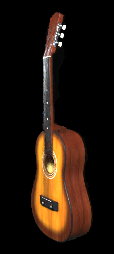
\includegraphics[width=0.062\textwidth]{figures/results/stat_set/valid/guitar4_imnrf_119k.png} & 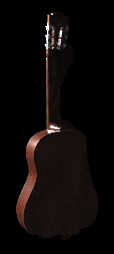
\includegraphics[width=0.062\textwidth]{figures/results/stat_set/valid/guitar8_imnrf_119k.png}
        \end{tabular}
        &
        \begin{tabular}{cc}
            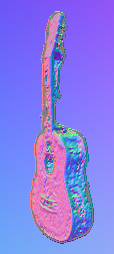
\includegraphics[width=0.062\textwidth]{figures/results/stat_set/valid/guitar4_imnrf_normal_119k.png} & 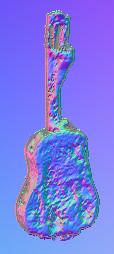
\includegraphics[width=0.062\textwidth]{figures/results/stat_set/valid/guitar8_imnrf_normal_119k.png}
        \end{tabular}
        &
        \begin{tabular}{cc}
            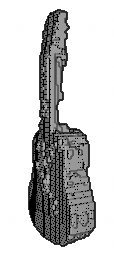
\includegraphics[width=0.062\textwidth]{figures/results/stat_set/valid/guitar4_imnrf_voxel_119k.png} & 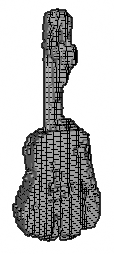
\includegraphics[width=0.062\textwidth]{figures/results/stat_set/valid/guitar8_imnrf_voxel_119k.png}
        \end{tabular}
        &
        %%%%% HOTDOG_IMNRF %%%%%
        &
        \begin{tabular}{cc}
            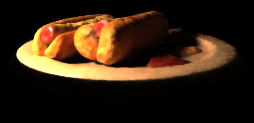
\includegraphics[width=0.124\textwidth]{figures/results/stat_set/valid/hotdog8_imnrf_45k.png} \\[-6pt]
            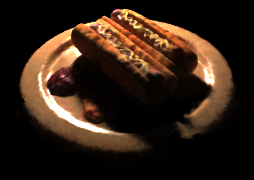
\includegraphics[width=0.124\textwidth]{figures/results/stat_set/valid/hotdog10_imnrf_45k.png}
        \end{tabular}
        &
        \begin{tabular}{cc}
            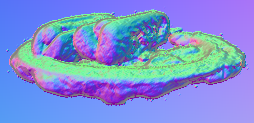
\includegraphics[width=0.124\textwidth]{figures/results/stat_set/valid/hotdog8_imnrf_normal_45k.png} \\[-6pt]
            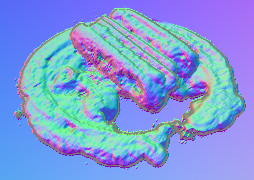
\includegraphics[width=0.124\textwidth]{figures/results/stat_set/valid/hotdog10_imnrf_normal_45k.png}
        \end{tabular}
        &
        \begin{tabular}{cc}
            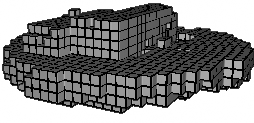
\includegraphics[width=0.124\textwidth]{figures/results/stat_set/valid/hotdog8_imnrf_voxel_45k.png} \\[-6pt]
            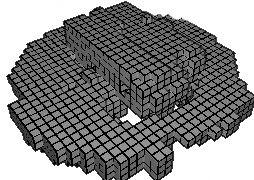
\includegraphics[width=0.124\textwidth]{figures/results/stat_set/valid/hotdog10_imnrf_voxel_45k.png}
        \end{tabular} 
        &
        \rot{ImNRF}
        \\ [-2pt]
        
        
        %%%%%%%%%%%%%%%%%%%
        %%%%% LEGOS %%%%%%%
        %%%%%%%%%%%%%%%%%%%
        Target & Output & Normal & Voxel  &  Target & Output & Normal & Voxel &\\

        %%%%% LEGO0_EXVA %%%%%
        %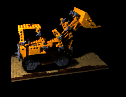
\includegraphics[width=0.124\textwidth]{figures/results/stat_set/valid/lego0_exva_55k.png}
        &
        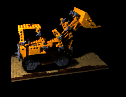
\includegraphics[width=0.124\textwidth]{figures/results/stat_set/valid/lego0_exva_55k.png}
        &
        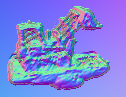
\includegraphics[width=0.124\textwidth]{figures/results/stat_set/valid/lego0_exva_normal_55k.png}
        &
        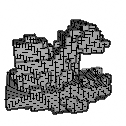
\includegraphics[width=0.124\textwidth]{figures/results/stat_set/valid/lego0_exva_voxel_55k.png}
        &
        %%%%% LEGO2_EXVA %%%%%
        %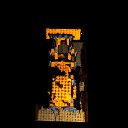
\includegraphics[width=0.124\textwidth]{figures/results/stat_set/valid/lego2_nsvf_57k.png}
        &
        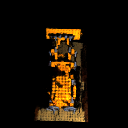
\includegraphics[width=0.124\textwidth]{figures/results/stat_set/valid/lego2_exva_55k.png}
        &
        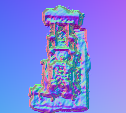
\includegraphics[width=0.124\textwidth]{figures/results/stat_set/valid/lego2_exva_normal_55k.png}
        &
        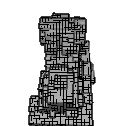
\includegraphics[width=0.124\textwidth]{figures/results/stat_set/valid/lego2_exva_voxel_55k.png} 
        &
        \rot{ExVA}
        \\[-5pt]

        %%%%% LEGO0_NSVF %%%%%
        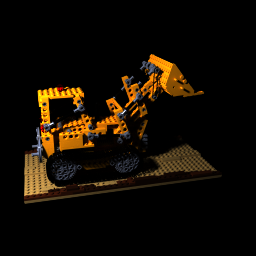
\includegraphics[width=0.124\textwidth]{figures/results/stat_set/valid/lego0_targ_256px.png}
        &
        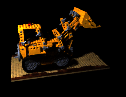
\includegraphics[width=0.124\textwidth]{figures/results/stat_set/valid/lego0_nsvf_57k.png}
        &
        \includegraphics[width=0.124\textwidth]{figures/results/stat_set/valid/lego0_nsvf_normal_57k.png}
        &
        \includegraphics[width=0.124\textwidth]{figures/results/stat_set/valid/lego0_nsvf_voxel_57k.png}
        &
        %%%%% LEGO2_NSVF %%%%%
        \includegraphics[width=0.124\textwidth]{figures/results/stat_set/valid/lego2_targ_256px.png}
        &
        \includegraphics[width=0.124\textwidth]{figures/results/stat_set/valid/lego2_nsvf_57k.png}
        &
        \includegraphics[width=0.124\textwidth]{figures/results/stat_set/valid/lego2_nsvf_normal_57k.png}
        &
        \includegraphics[width=0.124\textwidth]{figures/results/stat_set/valid/lego2_nsvf_voxel_57k.png} 
        &
        \rot{NSVF}
        \\[-5pt]

        %%%%% LEGO0_IMNRF %%%%%
        %\includegraphics[width=0.124\textwidth]{figures/results/stat_set/valid/lego0_exva_55k.png}
        &
        \includegraphics[width=0.124\textwidth]{figures/results/stat_set/valid/lego0_imnrf_45k.png}
        &
        \includegraphics[width=0.124\textwidth]{figures/results/stat_set/valid/lego0_imnrf_normal_45k.png}
        &
        \includegraphics[width=0.124\textwidth]{figures/results/stat_set/valid/lego0_imnrf_voxel_45k.png}
        &
        %%%%% LEGO2_IMNRF %%%%%
        %\includegraphics[width=0.124\textwidth]{figures/results/stat_set/valid/lego2_nsvf_57k.png}
        &
        \includegraphics[width=0.124\textwidth]{figures/results/stat_set/valid/lego2_imnrf_45k.png}
        &
        \includegraphics[width=0.124\textwidth]{figures/results/stat_set/valid/lego2_imnrf_normal_45k.png}
        &
        \includegraphics[width=0.124\textwidth]{figures/results/stat_set/valid/lego2_imnrf_voxel_45k.png} 
        &
        \rot{ImNRF}
        \\[-5pt]
        

    \end{tabular*}
    \caption{The overview of some novel view synthesis results
    achieved with \textit{ExVA}, \textit{NSVF} and \textit{ImNRF}
    methods trained on static light datasets.
    Columns correspond to the output maps.
    Normal map is calculated from the sigma-field predicted by the model.
    Note how all schemes fail to learn geometry in the shadowed regions.
    It can also be seen how more the \textit{ExVA} method is sensitive
    to inconsistent geometry comparing with the \textit{NSVF} renders.
    The \textit{ImNRF} and \textit{NSVF} methods shows almost equal performance.
    }
    
    % \im{static results for ImNF: lego256 u4110, hotdog256 u4109, guitar256 u4101}
    \label{fig:static_valid_results}
\end{figure}
\endgroup